\documentclass[10pt,a4paper]{article}
\usepackage[utf8]{inputenc}
\usepackage[parfill]{parskip}
\usepackage[section]{placeins}
\usepackage{graphicx}
\usepackage{array}
\usepackage{tikz}
\usepackage{apacite}
\usepackage{url}

\title{{\Huge Sentiment Analysis for Social Media Comments}}
\author{Christoph Emunds, Benedikt Heinrichs, Dominik Nerger, Richard Polzin}
\date{\today}

\begin{document}
	\maketitle
	
	\begin{abstract}
	Analyzing customer experience offers valuable data for Business Intelligence. Especially in e-commerce, where users write reviews about products and services, the analysis of the customers' sentiment towards these entities yields significant insights into potential strengths and weaknesses of the product or service.

	Our work focuses on evaluating customer experience through the application of aspect-based sentiment analysis on social media posts. The data set contains a year's worth of Facebook comments on the pages of two supermarket chains (Tesco and Sainsbury). The goal is to extract as many triplets (e, a, s) as possible, where e is an entity (product or service), a is an aspect of this entity (performance, battery, politeness, etc.), and s is the sentiment polarity label (negative, neutral, positive).

	To accomplish this task, many different subtasks need to be solved. After a rudimentary preprocessing routine, the posts need to be POS tagged, Named Entity Recognition (NER) must be applied and sentiment words need to be detected and evaluated. During these tasks we face many challenges, as a significant number of social media texts do not follow the grammatical rules or contain a lot of misspellings. With the completed analysis we identify potential products and services, their corresponding aspects and sentiment words, which are scored and aggregated into an opinion.

	The results obtained from this analysis are visualized to get a better understanding of the customers' feelings towards these products, services, and their aspects. The visualization supports businesses in a wide range of decisions, such as product positioning and pricing. This can lead to better customer satisfaction, faster reactions to trends and overall revenue growth.
	\end{abstract}
	
	\newpage
	\tableofcontents
	\newpage

	\section{Introduction}
	In today's world, Social Media is a big part of the social life. On social networks like Facebook, besides personal accounts there are corporate accounts as well, with the possibility of customers/people interacting with companies, celebrities, sports teams etc.
	People can review companies or comment on their news feed, allowing interaction between the two entities. These comments or reviews are often filled with positive or negative sentiments because they mostly occur after a really positive or negative experience with the company. Through the comments, it should therefore be possible to extract sentiments about products or aspects of the company.
	The project presented in this document focuses on finding and analyzing customers' opinions on products and their aspects from social media posts of a supermarket chain. This report describes the required background knowledge and the related work that we build upon. We present how we used the available components to try and fulfill our task. For this task we review the previously defined research questions and evaluate their success or failure.
	
	\section{Related work}
		
		\subsection{POS-Tagging}
		POS-Tagging (part-of-speech tagging), also called grammatical tagging or word-category disambiguation, refers to the process of identifying particular parts of speech like nouns or verbs. 

		Identifying the role of a certain word within a sentence is important for the task of sentiment analysis, as identifying entities and their corresponding aspects can be handled much easier relying on certain assumptions about the part of speech of words.

		Frequent nouns or noun phrases often describe aspects of products and the vocabulary that is used to describe those usually converges. With such an approach many important aspects can easily be found, but on a more general scheme grammatical based relationships can be used to extract important aspects.

		For example words that express opinion on something, like 'great' or 'bad' can be incorporated in rules to extract aspects. To sum it up POS-Tagging is an important part of sentiment analysis.
		
		While being important POS-Tagging is also a complex problem. Word-forms in natural language are often ambiguous. For example the word 'dogs' is usually thought of as a plural noun, but can be used as a verb as well:

		\begin{quote}
			The sailor dogs the hatch.
		\end{quote}

		Due to the complexity, machine learning techniques are often applied in POS-Taggers. Popular approaches such as the Viterbi algorithm, the Brill tagger or the Baum-Welch algorithm work with techniques such as dynamic programming, supervised learning or hidden Markov models.
		
		\subsection{NER-Tagging}
		
		Named-Entity recognition (NER) is a task that seeks to locate and classify specific information in text. This information is called a named entity and can refer to categories such as the names of persons, locations, times or many others.

		An annotated sentence could look like this :

		\begin{quote}
			[Tim Cook]$_{[Person]}$ has a Net worth of [785 million USD]$_{[Monetary Value]}$ as of [March 16. 2017]$_{[Time]}$.
		\end{quote}
		
		Often the task of NER-Tagging is separated into two. In the first part names are detected and in the second part these names are classified. 
		
		While state-of-the-art NER-Taggers perform very well and produce near-human performance they are also brittle and do not perform well in domains they were not designed for.
	
	\section{Approach}
		\subsection{Preprocessing}
	
		We pre-processed the data by extracting the actual text of the posts into separate files, which can be processed by SyntaxNet. We decided to exclude posts that are less than 20 characters long or include images. This is due to the fact that posts which are too short do not yield much information most of the time. Furthermore, posts that include images often refer to objects in the image, which makes it hard to understand the author's sentiment without analyzing the image content.
	
		\subsection{Extracting entities and aspects}
		POS-tagging and Named Entity Extraction with OpenNLP

		First, we identify frequent nouns and noun phrases with a POS-Tagger. Since people commenting on aspects of a product usually use a limited vocabulary, this process should yield a first set of possible entities and aspects. The frequency threshold needs to be chosen experimentally.

		\subsection{Determining sentiment polarities}
		nltk's Vader module
		Specifically developed for social media

	\section{Results}
		The overall goal is to extract as many quintuples $(e_i, a_{ij}, s_{ijkl}, h_k, t_l)$ as possible, where $e_i$ is the $i$'th entity and $a_{ij}$ is the $j$'th aspect of entity $i$ the opinion is expressed on. $s_{ijkl}$ is the sentiment polarity, which can take on the values \textit{positive} or \textit{negative}. $h_k$ describes the opinion holder and $t_l$ the time at which the opinion was expressed.

		\subsection{Visualization}
		We will use the sentiment lexicon by \cite{Hu:2004:MSC:1014052.1014073}, which includes mis-spellings, morphological variants, slang and social-media mark-up of 2006 positive and 4783 negative words.

		Because it is time consuming to take the results and derive a meaning from them by hand, we decided to visualize the results in a web application. On the server side, we use Python with the library Flask. On the client side, we use the JavaScript libraries d3.js, vue.js and jQuery.
	
		For the visualization, we use the \textit{JSON} file containing the aggregated opinions that are the result of executing the pipeline as well as a \textit{JSON} containing the positive and negative sentiment words that are provided by the lexicon-based sentiment analysis.
	
		The data is visualized with each product having its own page that is loaded from a dropdown menu and each aspect of the product being visualized with a bar chart as well as the specific posts being shown below the bar chart. The bar chart can be seen in Figure~\ref{fig:barchart}. It shows the amount of negative, neutral and positive sentiments regarding the combination of product and aspect.
	
		\begin{figure}[h]
			\centering
			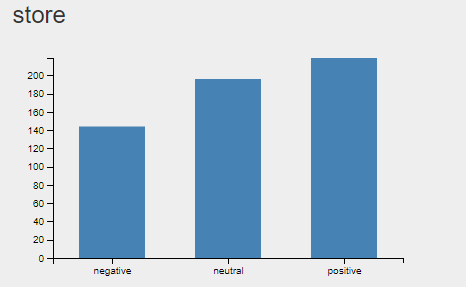
\includegraphics[width=0.7\linewidth]{data/barchart}
			\caption{Bar chart displaying the sentiments regarding the customer service with aspect 'store'}
			\label{fig:barchart}
		\end{figure}
			
		An excerpt of posts regarding the combination of product and aspect is shown below each bar chart, with a maximum of 10 posts per aspect. In Figure~\ref{fig:posts}, the highlighted posts can be seen. Positive and negative sentiments are highlighted in colors green and red, respectively. Mentions of the product are highlighted in orange and the aspect is shown with a cyan highlighting.
			
		\begin{figure}[h]
			\centering
			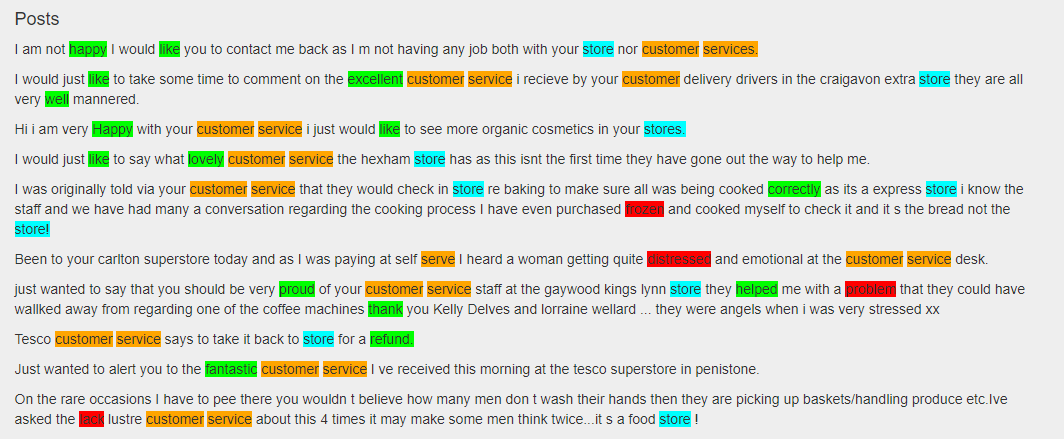
\includegraphics[width=0.9\linewidth]{data/posts}
			\caption{Highlighted posts regarding the customer service with aspect 'store'}
			\label{fig:posts}
		\end{figure}
	
	\section{Discussion and Conclusion}
	
	\section{Appendix}
	%TODO: Make proper appendix, don't know the commands from the top of my head
		
		\subsection{Using the code}
		To reproduce our work, the provided code has to be executed in a certain sequence. The following will talk about the needed steps.

	\newpage

	\bibliography{rp}
	\bibliographystyle{apacite}
\end{document}